\chapter{Técnicas de laboratorio III: la práctica de la investigación}\label{ch:b3:lab-techniques-3}

Un frasco de disolución de butillitio se inflama si una gota toca el aire; una
\omterm{def:b3:lab-techniques-3:schlenk}{caja de guantes} mantiene el oxígeno y el agua por debajo de unas pocas partes por millón para que esos
compuestos puedan pesarse como la sal de mesa. La química de investigación suele empezar
dejando fuera la atmósfera, y termina con una afirmación que otros deben poder
comprobar: un compuesto nuevo, con su estructura y su pureza demostradas por varios métodos
independientes, y sus datos registrados y publicados para que el trabajo pueda repetirse. Este
último capítulo reúne la práctica de la investigación: la manipulación de sustancias sensibles
al aire, la caracterización de un compuesto nuevo, la valoración estadística de un resultado,
el \omterm{def:b3:lab-techniques-3:notebook}{cuaderno de laboratorio} y la lectura de la bibliografía, y la evaluación de los riesgos de un
procedimiento que nadie ha realizado antes.

\begin{recall}
El volumen del primer año trató los peligros, los riesgos, los pictogramas, las indicaciones H y P, las fichas
de datos de seguridad y la incertidumbre de medida con sus evaluaciones de tipo A y B; el
volumen del segundo año, las atmósferas inertes, el tratamiento, los agentes desecantes, la cromatografía flash,
la espectrometría de masas (HRMS, masa monoisotópica), la RMN de $^{13}$C, los intervalos de confianza,
el coeficiente de Student, la calibración, la precisión, la veracidad, el sesgo, la repetibilidad,
la validación de métodos, el aumento adiabático de temperatura y la reacción térmica descontrolada.
Los \cref{ch:b3:advanced-nmr}, \cref{ch:b3:x-ray-diffraction} y
\cref{ch:b3:electrode-kinetics} aportaron los métodos estructurales y
electroquímicos.
\end{recall}

\begin{omfigure}
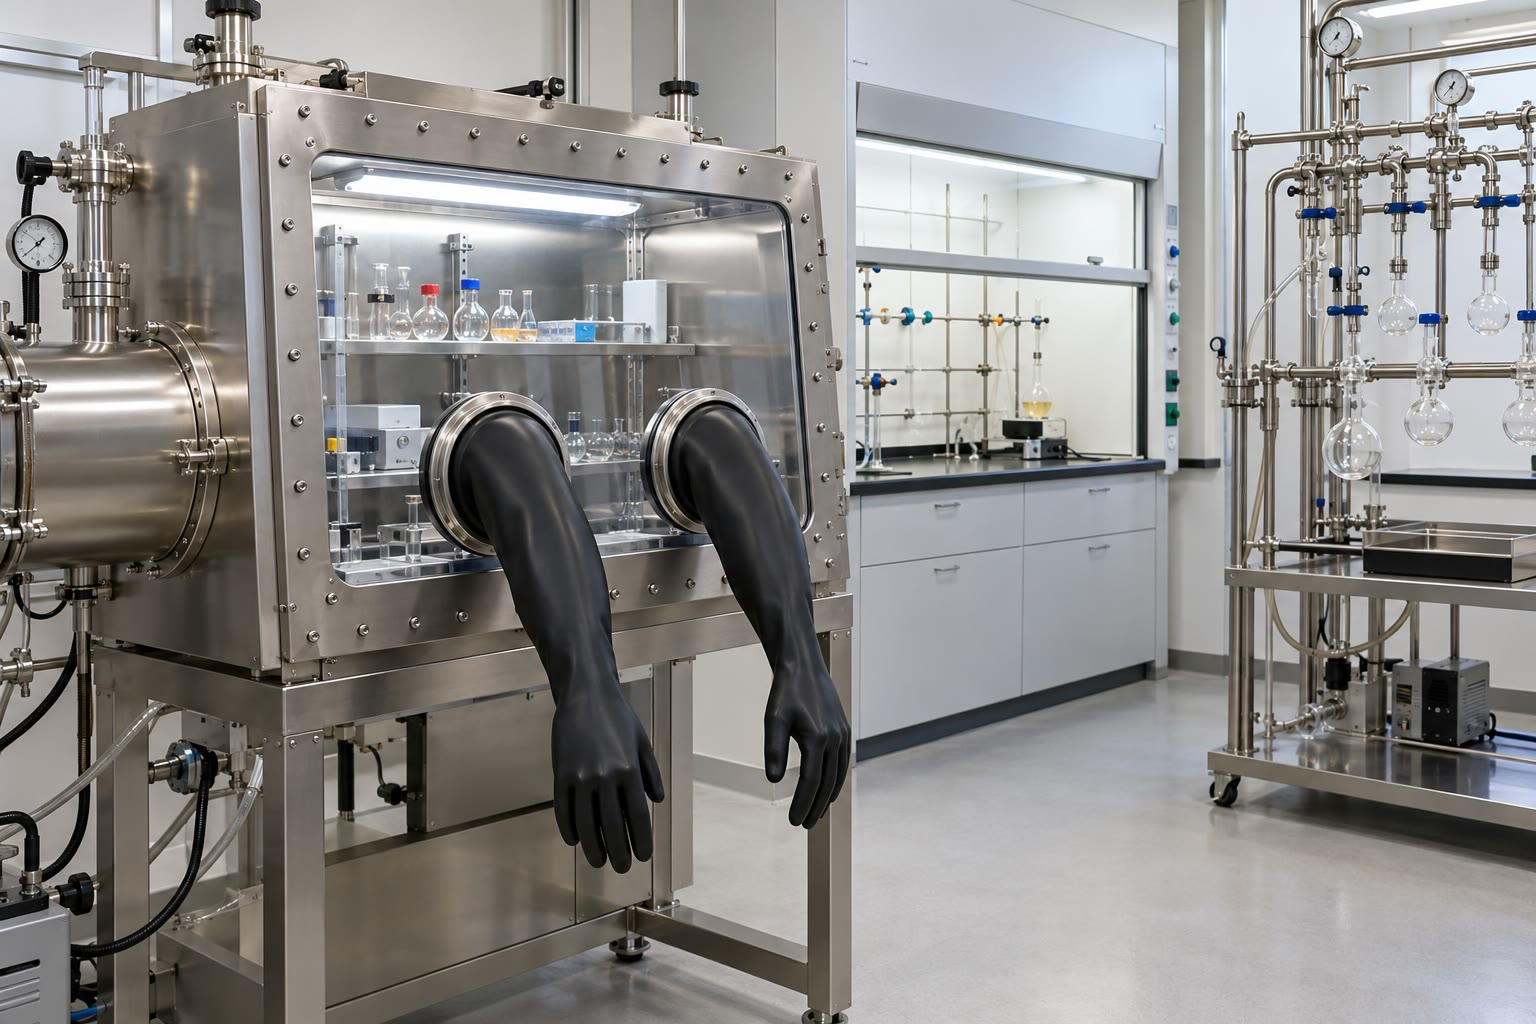
\includegraphics[width=0.58\linewidth]{images/book4/ai/b3-33-glovebox.jpg}

{\small Un laboratorio de investigación con una \omterm{def:b3:lab-techniques-3:schlenk}{caja de guantes}: la caja de acero inoxidable, llena
de nitrógeno o de argón secos, se maneja a través de los guantes; el cilindro de la
izquierda es la antecámara para introducir y sacar objetos.}
\end{omfigure}

\section{Trabajar sin aire}

\begin{definition}[Compuestos sensibles al aire]\label{def:b3:lab-techniques-3:air-sensitive}
Un \emph{compuesto sensible al aire}\index{compuesto sensible al aire} reacciona con el
dioxígeno o con el agua del aire, y se descompone o pierde su actividad. Una
\emph{sustancia pirofórica}\index{sustancia piroforica@sustancia pirofórica} se inflama espontáneamente en
el aire.
\end{definition}

\begin{definition}[Línea de Schlenk y caja de guantes]\label{def:b3:lab-techniques-3:schlenk}
Una \emph{línea de Schlenk}\index{linea de Schlenk@línea de Schlenk} es un doble colector de vidrio: un tubo
conectado a una bomba de vacío a través de una trampa fría, y el otro a un suministro de gas inerte
seco que sale a través de un borboteador de aceite, con llaves que conectan cada salida a
uno u otro. Un \emph{matraz de Schlenk}\index{matraz de Schlenk} tiene un brazo lateral con una llave
para conectarlo a la línea. Una \emph{caja de guantes}\index{caja de guantes} es una caja estanca
llena de gas inerte, purificado de forma continua, en la que se trabaja a través de
guantes.
\end{definition}

\begin{omfigure}
\begin{tikzpicture}[font=\scriptsize, >=Stealth]
  % manifolds
  \draw[om glass, line width=1.1pt] (0,3.0) -- (8.0,3.0);
  \draw[om glass, line width=1.1pt] (0,2.5) -- (8.0,2.5);
  \node[anchor=east] at (-1.0,3.0) {gas inerte};
  \node[anchor=east] at (0,2.5) {vacío};
  % taps
  \foreach \x in {2.0,4.0,6.0} {
    \draw[om glass] (\x,3.0) -- (\x,2.5);
    \draw[fill=white] (\x,2.75) circle (0.12);
    \draw (\x-0.1,2.75) -- (\x+0.1,2.75);
    \draw[om glass] (\x,2.5) -- (\x,2.0);
  }
  % flask on the middle tap
  \draw[thick, black!60] (4.0,2.0) -- (4.0,1.6) -- (4.6,1.6);
  \pic[scale=0.5, transform shape] at (5.0,-0.2) {rbflask={0.3}{omDef!20}};
  \draw[om glass] (4.6,1.6) -- (4.9,1.25);
  \node[anchor=west] at (5.4,0.4) {matraz de Schlenk};
  % bubbler at the gas end
  \pic[scale=0.55, transform shape] at (8.9,1.5) {bubbler};
  \draw[om glass] (8.0,3.0) -- (8.6,3.0) -- (8.6,2.9);
  \node[anchor=west] at (9.4,2.2) {borboteador de aceite};
  % trap and pump at the vacuum end
  \draw[om glass] (0.4,2.5) -- (0.4,1.6);
  \draw[om glass, fill=omDef!8] (0.15,1.6) rectangle (0.65,0.4);
  \fill[omDef!25] (0.0,0.2) rectangle (0.8,1.2);
  \node[anchor=north] at (0.4,0.2) {trampa fría};
  \draw[om glass] (0.65,0.9) -- (1.6,0.9);
  \draw[fill=black!15] (1.6,0.6) rectangle (2.6,1.2);
  \node at (2.1,0.9) {bomba};
  \draw[->, thick] (-0.9,3.0) -- (0,3.0);
\end{tikzpicture}

{\small Una \omterm{def:b3:lab-techniques-3:schlenk}{línea de Schlenk}, en esquema: un colector de gas y un colector de vacío unidos por
llaves; cada llave conecta su matraz al vacío o al gas inerte. El vapor de disolvente
extraído por bombeo se condensa en la trampa fría antes de llegar a la bomba; el gas sale
a través de un borboteador de aceite, que impide que el aire entre en sentido contrario.}
\end{omfigure}

\begin{proposition}[Ciclos de vacío y llenado]\label{prop:b3:lab-techniques-3:purge-cycles}
Si un matraz lleno de aire a la presión $p_0$ se evacua hasta $p_{\min}$ y se vuelve a llenar con
gas inerte puro, $n$ veces, la fracción de aire original que queda es $(p_{\min}/p_0)^n$.
\end{proposition}

\begin{proof}
Evacuar hasta $p_{\min}$ deja una fracción $p_{\min}/p_0$ del gas, de la misma composición; el
llenado con gas inerte puro restablece $p_0$ sin añadir aire. Cada ciclo multiplica la
fracción de aire por $p_{\min}/p_0$; al cabo de $n$ ciclos, $(p_{\min}/p_0)^n$.
\end{proof}

Tres ciclos hasta \qty{0.1}{mbar} dejan, sobre el papel, $10^{-12}$ del aire; en la práctica, las fugas, el gas
adsorbido en el vidrio y la desgasificación de la grasa y de los septos fijan el límite, por lo que
el material de vidrio se seca en una estufa y se monta en caliente.

\begin{definition}[Transferencia con cánula]\label{def:b3:lab-techniques-3:cannula}
Una \emph{transferencia con cánula}\index{transferencia con canula@transferencia con cánula} lleva un líquido sensible al aire
de un recipiente cerrado a otro a través de una aguja larga de doble punta, impulsado
por una pequeña sobrepresión de gas inerte en el primer recipiente.
\end{definition}

\begin{omfigure}
\begin{tikzpicture}[font=\scriptsize, >=Stealth]
  \pic at (0,0) {rbflask={0.35}{omThm!25}};
  \pic at (4.2,0) {rbflask={0.1}{omDef!15}};
  \pic at (0,3.0) {septum};
  \pic at (4.2,3.0) {septum};
  \draw[black!70, line width=0.9pt] (0.05,0.25) -- (0.05,3.5) to[out=90, in=90] (4.15,3.5) -- (4.15,1.6);
  \draw[->, thick, omThm] (1.3,3.95) -- (2.9,3.95) node[midway, above] {líquido};
  \draw[->, thick] (-1.3,3.4) -- (-0.15,3.2) node[pos=0, left] {entrada de gas inerte (ligera sobrepresión)};
  \draw[->, thick] (4.35,3.2) -- (5.4,3.6) node[right] {salida al borboteador};
  \node[anchor=north] at (0,-0.1) {origen};
  \node[anchor=north] at (4.2,-0.1) {receptor};
\end{tikzpicture}

{\small Una \omterm{def:b3:lab-techniques-3:cannula}{transferencia con cánula}: la punta inferior de la cánula se sumerge en el líquido del
matraz de origen; el gas inerte que se deja entrar en el matraz de origen empuja el líquido a través de la
cánula hacia el receptor, que se ventila a través de una aguja conectada al borboteador.}
\end{omfigure}

\begin{method}[Una transferencia con cánula]\label{met:b3:lab-techniques-3:cannula}
\begin{enumerate}
  \item Poner los dos matraces, cerrados con septos, bajo gas inerte en la \omterm{def:b3:lab-techniques-3:schlenk}{línea de Schlenk}.
  \item Purgar la cánula con gas: introducir un extremo en el matraz de origen por encima del líquido
        hasta que salga gas por el otro extremo, e introducir entonces ese extremo en el receptor.
  \item Ventilar el receptor con una aguja; hundir el extremo de la cánula del lado del origen por debajo de la
        superficie del líquido: la sobrepresión hace pasar el líquido.
  \item Para detenerlo, levantar la punta por encima del líquido; retirar primero la cánula del receptor
        y enjuagarla enseguida con un disolvente seco y después con agua, en la vitrina.
\end{enumerate}
\end{method}

\begin{definition}[Desgasificación por congelación, vacío y descongelación]\label{def:b3:lab-techniques-3:degassing}
La \emph{desgasificación por congelación, vacío y descongelación}\index{desgasificacion por congelacion, vacio y descongelacion@desgasificación por congelación, vacío y descongelación} elimina
los gases disueltos de un líquido congelándolo en nitrógeno líquido, evacuando el
espacio situado encima, cerrando la llave y dejándolo descongelar, de modo que el gas disuelto escape
hacia el vacío; el ciclo se repite tres veces.
\end{definition}

Los disolventes secos se obtienen hoy de columnas de alúmina activada bajo gas inerte,
en lugar de destilarlos sobre sodio. Las disoluciones de organolíticos pierden concentración con el
tiempo y se valoran antes de usarlas, por ejemplo frente a una cantidad pesada de
ácido difenilacético en THF seco: el primer equivalente desprotona el ácido, y la
primera gota en exceso da el dianión amarillo.

\begin{proposition}[Título de un organolítico]\label{prop:b3:lab-techniques-3:titre}
Si una masa $m$ de ácido difenilacético (masa molar $M$) necesita un volumen $V$ de una
disolución de organolítico para alcanzar el viraje, la concentración es $c = m/(MV)$.
\end{proposition}

\begin{proof}
Hasta el punto final, cada organolítico arranca un protón del ácido; el
color aparece cuando el ácido se ha consumido. Las cantidades son iguales: $cV = m/M$.
\end{proof}

\begin{inthelab}[La antecámara de la caja de guantes]
Los objetos entran en una \omterm{def:b3:lab-techniques-3:schlenk}{caja de guantes} a través de su antecámara: se colocan dentro, se
cierra la puerta exterior y la cámara se evacua y se vuelve a llenar con el gas de la caja
tres veces, con una evacuación final larga para los objetos porosos, que retienen aire;
solo entonces se abre la puerta interior desde dentro de la caja con los guantes. Nunca se bombean en la antecámara
disolventes ni recipientes abiertos de líquidos volátiles, y
nada que pudiera envenenar el purificador (tioles, disolventes halogenados) se abre
dentro sin autorización.
\end{inthelab}

\begin{omfigure}
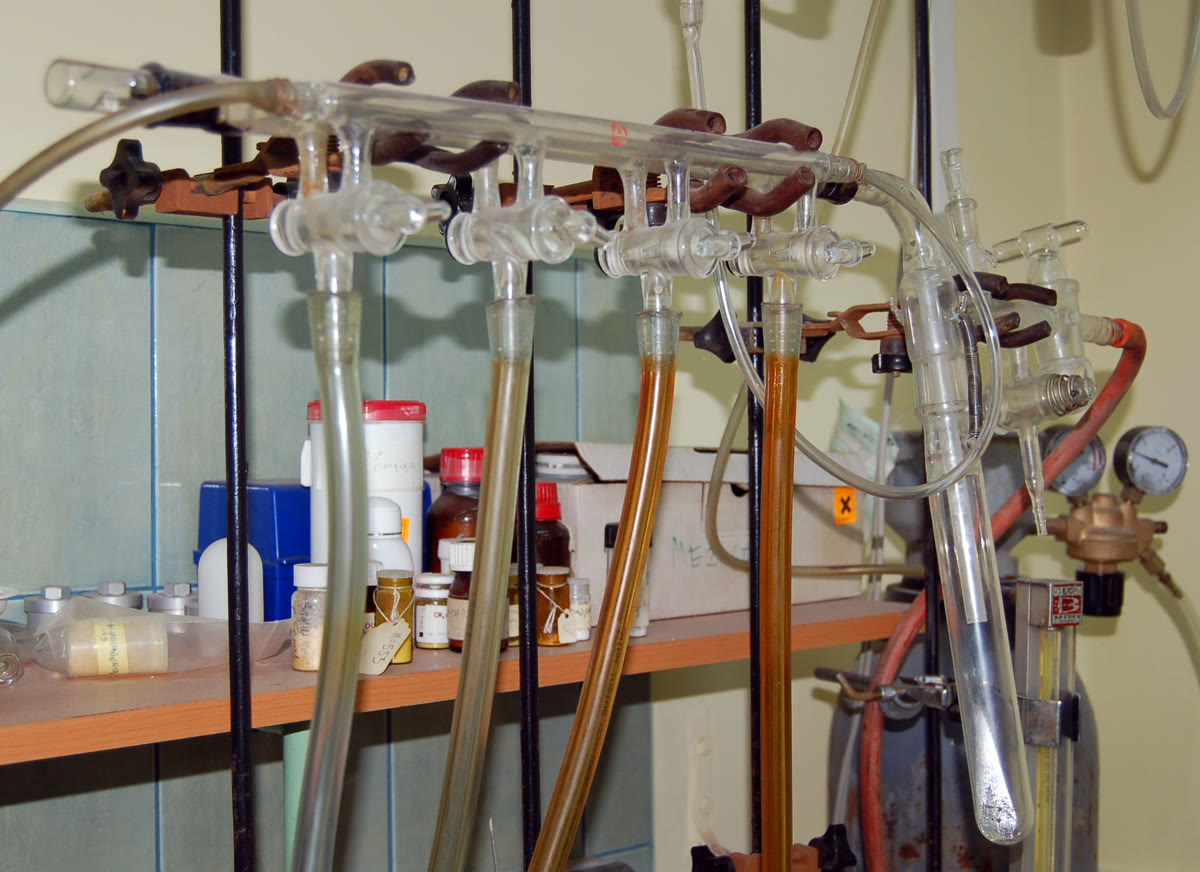
\includegraphics[width=0.46\linewidth]{images/book4/schlenk-line.jpg}

{\small Una \omterm{def:b3:lab-techniques-3:schlenk}{línea de Schlenk} en uso: el colector de vidrio con sus llaves, los tubos hacia los
matraces y el regulador de gas. Fotografía: Polimerek, CC BY-SA 3.0.}
\end{omfigure}

\section{Caracterizar un compuesto nuevo}

\begin{method}[Caracterizar un compuesto nuevo]\label{met:b3:lab-techniques-3:characterise}
\begin{enumerate}
  \item Pureza: una sola mancha en CCF con dos eluyentes, un solo pico en HPLC o en CG, un punto de fusión
        neto; \omterm{def:b3:lab-techniques-3:qnmr}{RMN cuantitativa} si se necesita una pureza másica.
  \item Fórmula: HRMS dentro de unas pocas ppm de la masa calculada, y el patrón
        isotópico; o \omterm{def:b3:lab-techniques-3:elemental}{análisis elemental}.
  \item Estructura: RMN de $^1$H y de $^{13}$C con experimentos 2D para las conectividades
        (\cref{ch:b3:advanced-nmr}), IR para los grupos funcionales; una estructura de rayos X de
        monocristal cuando crecen cristales (\cref{ch:b3:x-ray-diffraction}).
  \item Estereoquímica: NOE, constantes de acoplamiento, rotación óptica, ee por cromatografía
        quiral.
  \item Dar cada dato con sus condiciones, y los espectros en la \omterm{def:b3:lab-techniques-3:literature}{información
        complementaria}.
\end{enumerate}
\end{method}

\begin{omfigure}
\begin{tikzpicture}[font=\scriptsize, >=Stealth,
  box/.style={draw, rounded corners, align=center, fill=omDef!8, inner sep=3pt, minimum height=8mm}]
  \node[box] (a) at (0,0) {compuesto nuevo\\ aislado};
  \node[box] (b) at (2.85,0) {¿puro?\\ CCF, HPLC, p.f.};
  \node[box] (c) at (5.85,0) {fórmula\\ HRMS, CHN};
  \node[box] (d) at (8.75,0) {estructura\\ RMN (1D, 2D), IR};
  \node[box] (e) at (8.75,-1.6) {rayos X si hay cristales,\\ estereoquímica};
  \node[box, fill=omMeth!12] (f) at (5.85,-1.6) {¿coherente?\\ informe con los\\ datos brutos};
  \node[box, fill=omThm!10] (g) at (2.85,-1.6) {purificar de nuevo\\ (cromatografía,\\ cristalización)};
  \draw[->, thick] (a) -- (b); \draw[->, thick] (b) -- node[above, inner sep=1pt] {sí} (c);
  \draw[->, thick] (c) -- (d); \draw[->, thick] (d) -- (e); \draw[->, thick] (e) -- (f);
  \draw[->, thick] (b) -- node[left] {no} (g); \draw[->, thick] (g.north west) to[bend left=30] (a.south);
\end{tikzpicture}

{\small El flujo de trabajo de caracterización de un compuesto nuevo: primero la pureza, después la
fórmula y después la estructura; cada afirmación se apoya en al menos dos métodos
independientes, y los \omterm{def:b3:lab-techniques-3:notebook}{datos brutos} acompañan al informe.}
\end{omfigure}

\begin{definition}[Análisis elemental]\label{def:b3:lab-techniques-3:elemental}
El \emph{análisis elemental}\index{analisis elemental@análisis elemental} (análisis por combustión)
determina los porcentajes en masa de carbono, hidrógeno, nitrógeno y azufre de una
muestra quemándola en oxígeno y midiendo el dióxido de carbono, el agua, el
dinitrógeno y el dióxido de azufre formados.
\end{definition}

\begin{proposition}[Porcentajes en masa a partir de una fórmula]\label{prop:b3:lab-techniques-3:mass-fractions}
Para una fórmula $\mathrm{C}_a\mathrm{H}_b\mathrm{N}_c\dots$ de masa molar $M$, el porcentaje en masa de carbono es $100\,aA_r(\mathrm C)/M$, y del mismo modo
para los demás elementos.
\end{proposition}

\begin{proof}
Un mol de compuesto, de masa $M$, contiene $a$ moles de átomos de carbono, de masa $aA_r(\mathrm C)$;
la razón, multiplicada por 100, es el porcentaje en masa.
\end{proof}

% ledger: ea:tolerance, hrms:tolerance
La mayoría de las revistas de química piden valores de C, H y N encontrados a menos de 0.4 puntos
porcentuales de los calculados, o una medida de HRMS a menos de unas pocas ppm (5 ppm
para algunas), como prueba de la composición. Un amplio estudio interlaboratorios mostró que
incluso muestras puras incumplen el criterio de 0.4 con sorprendente frecuencia, un recordatorio de que un
criterio no es una ley de la naturaleza.

\begin{proposition}[Error en HRMS]\label{prop:b3:lab-techniques-3:ppm-error}
El error de una masa medida $m_{\mathrm{med}}$ respecto de la calculada $m_{\mathrm{calc}}$ es de
$10^6(m_{\mathrm{med}} - m_{\mathrm{calc}})/m_{\mathrm{calc}}$ ppm; para un ion, $m_{\mathrm{calc}}$ se calcula a partir de las masas monoisotópicas menos (o más) la
masa de los electrones arrancados (o añadidos).
\end{proposition}

\begin{proof}[Por definición]
El error en ppm es la diferencia relativa expresada en partes por millón; la
masa del ion difiere de la de la fórmula neutra en la de los electrones, \qty{5.486e-4}{u} cada uno, unas
pocas ppm para masas de unos cientos.
\end{proof}

\begin{definition}[RMN cuantitativa]\label{def:b3:lab-techniques-3:qnmr}
La \emph{RMN cuantitativa}\index{RMN cuantitativa} (qNMR) determina cantidades o
purezas a partir de las integrales de las señales, que son proporcionales al número de núcleos
cuando el espectro se registra con relajación completa entre pulsos, frente a un
patrón interno de pureza conocida pesado junto con la muestra.
\end{definition}

\begin{proposition}[Pureza por qNMR]\label{prop:b3:lab-techniques-3:qnmr}
Para una muestra de masa $m_x$ pesada con un patrón de masa $m_s$ y pureza $P_s$, con señales
de integrales $I_x$ e $I_s$ procedentes de $N_x$ y $N_s$ protones,
\[
  P_x = \frac{I_x}{I_s}\,\frac{N_s}{N_x}\,\frac{M_x}{M_s}\,\frac{m_s}{m_x}\,P_s.
\]
\end{proposition}

\begin{proof}
Las integrales son proporcionales a los números de protones: $I_x/I_s = (N_xn_x)/(N_sn_s)$. Con
$n_x = P_xm_x/M_x$ y $n_s = P_sm_s/M_s$, despejando $P_x$ se obtiene la fórmula.
\end{proof}

\begin{omfigure}
\begin{tikzpicture}
\begin{axis}[width=0.8\linewidth, height=5.0cm, x dir=reverse, xmin=3.0, xmax=7.0, ymin=-0.05, ymax=1.15, clip=false,
  axis x line=bottom, axis y line=none, xlabel={$\delta$ / ppm}, tick label style={font=\scriptsize}, label style={font=\small}]
\addplot[color=omDef, thick] table[x=ppm, y=y] {figdata/out/bachelor-3-qnmr.dat};
\node[font=\scriptsize, anchor=south] at (axis cs:6.09,0.33) {patrón, ArH (3 H)};
\node[font=\scriptsize, anchor=east] at (axis cs:4.20,0.98) {ferroceno (10 H)};
\node[font=\scriptsize, anchor=west, align=left] at (axis cs:3.72,0.70) {patrón,\\ $\ce{OCH3}$ (9 H)};
\end{axis}
\end{tikzpicture}

{\small Espectro sintético de protón de una muestra de ferroceno pesada con
1,3,5-trimetoxibenceno como patrón interno (modelo: 20.0 mg de muestra de pureza
98.0\,\% y 15.0 mg de patrón). Las integrales son proporcionales al número de
protones por la cantidad de cada compuesto; la razón entre el singlete del ferroceno y
el singlete aromático del patrón da la pureza.}
\end{omfigure}

\section{La estadística de un resultado de investigación}

\begin{definition}[Pruebas de significación]\label{def:b3:lab-techniques-3:tests}
Una \emph{prueba de significación}\index{prueba de significacion@prueba de significación} decide si unos datos son
compatibles con una \emph{hipótesis nula}\index{hipotesis nula@hipótesis nula}, normalmente la de que
no hay diferencia ni efecto, con un nivel elegido de riesgo de rechazarla
erróneamente (a menudo el 5\,\%).
\end{definition}

\begin{theorem}[Prueba $t$ para dos muestras]\label{thm:b3:lab-techniques-3:t-test}
Para dos series de $n_1$ y $n_2$ medidas independientes extraídas de distribuciones
normales de igual desviación típica, con medias $\bar x_1$, $\bar x_2$ y desviación típica
combinada $s_p$, el estadístico $t = (\bar x_1 - \bar x_2)/(s_p\sqrt{1/n_1 + 1/n_2})$ sigue la ley de Student con
$n_1 + n_2 - 2$ grados de libertad cuando las dos medias verdaderas son iguales. \admitted
\end{theorem}

\begin{proposition}[Prueba $F$]\label{prop:b3:lab-techniques-3:f-test}
Con las mismas hipótesis, la razón $F = s_1^2/s_2^2$ de dos varianzas muestrales sigue
la ley de Fisher con $(n_1 - 1, n_2 - 1)$ grados de libertad cuando las varianzas verdaderas son iguales.
\admitted
\end{proposition}

\begin{method}[¿Es mejor un nuevo rendimiento?]\label{met:b3:lab-techniques-3:compare-means}
\begin{enumerate}
  \item Repetir ambos procedimientos varias veces en las mismas condiciones; anotar
        todos los resultados.
  \item Comparar primero las dispersiones (prueba $F$); si son parecidas, combinarlas:
        $s_p^2 = [(n_1 - 1)s_1^2 + (n_2 - 1)s_2^2]/(n_1 + n_2 - 2)$.
  \item Calcular $t$ y comparar $|t|$ con el coeficiente de Student para $n_1 + n_2 - 2$ grados de
        libertad al nivel elegido.
  \item Mayor: la diferencia es significativa. Menor: los datos no muestran ninguna,
        lo que no demuestra que no exista.
\end{enumerate}
\end{method}

Un valor sospechoso nunca se suprime porque resulte incómodo. Las pruebas de valores atípicos
lo señalan, pero la decisión se basa en el cuaderno: una causa registrada (un error de
pesada, un matraz contaminado) justifica rechazarlo; sin ella, se conserva,
o se repite el experimento.

\section{El cuaderno, los datos de investigación y la bibliografía}

\begin{definition}[Cuaderno y datos brutos]\label{def:b3:lab-techniques-3:notebook}
El \emph{cuaderno de laboratorio}\index{cuaderno de laboratorio} es el registro fechado,
continuo e inalterado de los experimentos realizados, tal como se realizaron. Los \emph{datos
brutos}\index{datos brutos} son los registros originales de las medidas (ficheros de los
instrumentos, tiques de pesada, espectros) antes de cualquier tratamiento.
\end{definition}

\begin{method}[Redactar una entrada del cuaderno]\label{met:b3:lab-techniques-3:notebook}
\begin{enumerate}
  \item Fecha, título, objetivo y una referencia al experimento relacionado anterior.
  \item El esquema de reacción con las cantidades (masas, volúmenes, moles, equivalentes),
        el origen y los lotes de los reactivos, y la \omterm{def:b3:lab-techniques-3:assessment}{evaluación de riesgos}.
  \item Lo que se hizo y se observó, en orden y en el momento, incluido lo que salió
        mal; nunca borrar, sino tachar de modo que el original siga siendo legible.
  \item Resultados: rendimientos, nombres de los ficheros de \omterm{def:b3:lab-techniques-3:notebook}{datos brutos} y una conclusión; firmarla.
\end{enumerate}
\end{method}

\begin{definition}[Datos FAIR]\label{def:b3:lab-techniques-3:fair}
% ledger: fair:year
Los \emph{datos FAIR}\index{datos FAIR} son datos de investigación localizables,
accesibles, interoperables y reutilizables (según las siglas en inglés): descritos con metadatos ricos y un
identificador persistente, recuperables mediante protocolos normalizados, en formatos abiertos, con
una licencia y una procedencia claras.
\end{definition}

\begin{definition}[Integridad en la investigación]\label{def:b3:lab-techniques-3:integrity}
La \emph{integridad en la investigación}\index{integridad en la investigacion@integridad en la investigación} es la conducta y la
comunicación honestas y transparentes de la investigación. Sus vulneraciones más graves son la
\emph{fabricación}\index{fabricacion@fabricación} (inventar datos), la \emph{falsificación}\index{falsificacion@falsificación}
(alterar datos, imágenes o procedimientos) y el \emph{plagio}\index{plagio}
(presentar como propio el trabajo de otros).
\end{definition}

\begin{definition}[La bibliografía]\label{def:b3:lab-techniques-3:literature}
La \emph{literatura primaria}\index{literatura primaria} comunica investigación
original (artículos, patentes, tesis); la \emph{literatura
secundaria}\index{literatura secundaria} la revisa y la organiza (revisiones,
manuales, bases de datos), y los libros de texto forman una capa terciaria. La \emph{revisión
por pares}\index{revision por pares@revisión por pares} es la evaluación de un manuscrito por expertos independientes
antes de su publicación. La \emph{información complementaria}\index{informacion complementaria@información complementaria}
de un artículo contiene los detalles experimentales y los datos necesarios para
repetir y comprobar el trabajo.
\end{definition}

\begin{method}[Leer un procedimiento publicado]\label{met:b3:lab-techniques-3:read-paper}
\begin{enumerate}
  \item Leer la parte experimental y la \omterm{def:b3:lab-techniques-3:literature}{información complementaria}, no solo el
        resumen y el esquema.
  \item Comprobar la escala, las concentraciones, las temperaturas, los tiempos y el tratamiento; anotar
        lo que falta.
  \item Comprobar la caracterización de los productos frente al método anterior.
  \item Buscar artículos posteriores que hayan usado o corregido el procedimiento; realizarlo primero a
        pequeña escala.
\end{enumerate}
\end{method}

Las bases de datos de estructuras y de reacciones indexan la \omterm{def:b3:lab-techniques-3:literature}{literatura primaria} por compuesto y
por transformación, y se consultan dibujando una estructura o una reacción
en lugar de con palabras.

\section{Evaluación de riesgos de un procedimiento nuevo}

\begin{definition}[Evaluación de riesgos]\label{def:b3:lab-techniques-3:assessment}
Una \emph{evaluación de riesgos}\index{evaluacion de riesgos@evaluación de riesgos} de un procedimiento identifica sus
peligros, estima la probabilidad y la gravedad de los daños en las condiciones previstas,
y fija las medidas de control que reducen el riesgo a un nivel aceptable. La
\emph{jerarquía de controles}\index{jerarquia de controles@jerarquía de controles} los ordena de más a
menos eficaz: eliminación, sustitución, controles técnicos,
controles administrativos, equipos de protección individual.
\end{definition}

\begin{omfigure}
\begin{tikzpicture}[font=\scriptsize]
  \foreach \i/\lab/\col in {0/eliminación: suprimir el peligro/omMeth!40, 1/sustitución: un reactivo menos peligroso/omMeth!28, 2/técnicos: vitrina{,} caja de guantes{,} pantallas/omDef!22, 3/administrativos: procedimientos{,} formación/omProp!22, 4/equipos de protección individual/omThm!22} {
    \pgfmathsetmacro\w{5.4-0.95*\i}
    \fill[\col] ({-\w/2},{-0.75*\i}) -- ({\w/2},{-0.75*\i}) -- ({\w/2-0.475},{-0.75*\i-0.7}) -- ({-\w/2+0.475},{-0.75*\i-0.7}) -- cycle;
    \node[anchor=west] at (3.0,{-0.75*\i-0.35}) {\lab};
    \draw[black!30] ({\w/2-0.2},{-0.75*\i-0.35}) -- (2.95,{-0.75*\i-0.35});
  }
  \node[anchor=east, align=right] at (-2.9,-0.35) {más\\ eficaz};
  \node[anchor=east, align=right] at (-2.9,-3.35) {menos\\ eficaz};
  \draw[->, black!50] (-3.3,-0.85) -- (-3.3,-2.85);
\end{tikzpicture}

{\small La \omterm{def:b3:lab-techniques-3:assessment}{jerarquía de controles}, como una pirámide invertida: suprimir o sustituir
el peligro protege a todos, siempre; los equipos de protección solo protegen a quien
los lleva, y solo cuando los lleva y están intactos.}
\end{omfigure}

\begin{definition}[Formadores de peróxidos]\label{def:b3:lab-techniques-3:peroxide}
Un \emph{formador de peróxidos}\index{formador de peroxidos@formador de peróxidos} es un compuesto, como el éter
dietílico, el tetrahidrofurano o el 1,4-dioxano, que forma lentamente peróxidos explosivos
con el aire durante su almacenamiento, sobre todo una vez abierto y a la luz.
\end{definition}

\begin{method}[Evaluar los riesgos de un procedimiento nuevo]\label{met:b3:lab-techniques-3:risk-assessment}
\begin{enumerate}
  \item Enumerar todas las sustancias (reactivos, disolventes, productos, subproductos, gases
        liberados) con sus peligros según la ficha de datos de seguridad.
  \item Enumerar las operaciones y sus condiciones (calentamiento, presión, escala,
        extinción, residuos); estimar el calor liberado y el aumento adiabático de temperatura
        antes de cambiar de escala.
  \item Para cada peligro, elegir medidas de control descendiendo por la jerarquía; planificar la respuesta
        de emergencia (derrame, incendio, exposición) y la gestión de los residuos.
  \item Ponerlo por escrito, hacerlo revisar y revisarlo tras la primera realización.
\end{enumerate}
\end{method}

\begin{safety}{\ghs[0.62cm]{GHS02}\ghs[0.62cm]{GHS05}\ghs[0.62cm]{GHS07}\ghs[0.62cm]{GHS08}}
% ledger: ghs4:BuLi, ghs4:Et2O, ghs4:THF
Disoluciones de butillitio: pirofóricas, reaccionan violentamente con el agua liberando un
gas inflamable, provocan quemaduras graves; solo se manipulan bajo gas inerte, con un cubo de
arena seca a mano y sin agua cerca. El hidruro de sodio libera igualmente
hidrógeno con el agua y la humedad, y se usa en forma de dispersión en aceite. El éter
dietílico y el THF son \omterm{def:b3:lab-techniques-3:peroxide}{formadores de peróxidos} muy inflamables: se fechan al abrirlos, se comprueba
la presencia de peróxidos antes de destilarlos o evaporarlos, y se desechan según un calendario.
\end{safety}

\begin{history}[El material de vidrio de Schlenk]
Wilhelm Schlenk, que estudiaba los compuestos organoalcalinos y los radicales en la década de 1910,
diseñó los matraces y las técnicas que le permitieron manipularlos sin aire; la
línea y el matraz siguen llevando su nombre. Las primeras \omterm{def:b3:lab-techniques-3:schlenk}{cajas de guantes} se construyeron en la
década de 1940 para los materiales radiactivos, y pronto las adoptaron los químicos que trabajaban con
\omterm{def:b3:lab-techniques-3:air-sensitive}{compuestos sensibles al aire}.
\end{history}

\section{Ejercicios}

\begin{exercise}[$\star$]\label{exo:b3:lab-techniques-3:1}
Un matraz se evacua hasta \qty{0.50}{mbar} y se vuelve a llenar hasta \qty{1013}{mbar} con argón tres veces. ¿Qué fracción del
aire original queda, en teoría? ¿Qué limita realmente el resultado?
\end{exercise}

\begin{exercise}[$\star$]\label{exo:b3:lab-techniques-3:2}
Una disolución de butillitio tiene un título de \qty{1.48}{mol/L}. ¿Qué volumen hay que transferir para aportar
\qty{20.0}{mmol}?
\end{exercise}

\begin{exercise}[$\star$]\label{exo:b3:lab-techniques-3:3}
% ledger: mass:C12, mass:H1, mass:Fe56, const4:me.u, hrms:tolerance
Calcúlese la masa exacta del catión radical del ferroceno, $\ce{C10H10Fe+}$, a partir de las masas monoisotópicas
($^{12}$C, exactamente 12; $^1$H, 1.00782503; $^{56}$Fe, 55.93493633; electrón, \qty{5.486e-4}{u}), y el error de una medida de
186.0129 en ppm.
\end{exercise}

\begin{exercise}[$\star$]\label{exo:b3:lab-techniques-3:4}
Clasifíquense como \omterm{def:b3:lab-techniques-3:literature}{literatura primaria}, secundaria o terciaria: un artículo de revisión, un
artículo de revista que comunica una síntesis nueva, una patente, un manual de constantes
físicas, una tesis, un libro de texto.
\end{exercise}

\begin{exercise}[$\star\star$]\label{exo:b3:lab-techniques-3:5}
% ledger: ea:tolerance
Calcúlense los porcentajes en masa de C, H y N de la cafeína, $\ce{C8H10N4O2}$, y decídase si los valores
encontrados, C 49.31, H 5.22, N 28.71\,\%, cumplen el criterio habitual de 0.4 puntos.
\end{exercise}

\begin{exercise}[$\star\star$]\label{exo:b3:lab-techniques-3:6}
Una muestra de \qty{170.0}{mg} de ácido difenilacético ($\ce{C14H12O2}$) necesita \qty{0.54}{mL} de una disolución de butillitio para alcanzar
el punto final amarillo. Calcúlese el título.
\end{exercise}

\begin{exercise}[$\star\star$]\label{exo:b3:lab-techniques-3:7}
Un procedimiento antiguo daba rendimientos del 72, 75, 71, 74 y 73\,\%; uno modificado, del 76, 78, 75, 77 y
79\,\%. Con un coeficiente de Student de 2.31 para 8 grados de libertad al 95\,\% (datos del ejercicio),
¿es significativa la mejora?
\end{exercise}

\begin{exercise}[$\star\star$]\label{exo:b3:lab-techniques-3:8}
Dos métodos dan seis resultados cada uno, con desviaciones típicas de 0.80 y 0.30 (mismas
unidades). Con una $F$ crítica de 5.05 para (5, 5) grados de libertad al 95\,\% (datos del
ejercicio), ¿difieren sus precisiones?
\end{exercise}

\begin{exercise}[$\star\star$]\label{exo:b3:lab-techniques-3:9}
Propóngase un plan de almacenamiento y de control para los frascos de THF y de éter dietílico
de un laboratorio.
\end{exercise}

\begin{exercise}[$\star\star\star$]\label{exo:b3:lab-techniques-3:10}
Un estudiante prevé desprotonar un alcohol con hidruro de sodio en DMF a 60 °C a una
escala de 50 g. Identifíquense los peligros (incluidos los térmicos de este disolvente con
la base) y elíjanse medidas de control descendiendo por la jerarquía.
\end{exercise}

\begin{exercise}[$\star\star\star$]\label{exo:b3:lab-techniques-3:11}
Propáguense las incertidumbres típicas relativas de $I_x$, $I_s$ (0.50\,\% cada una), $m_x$ y $m_s$ (\qty{0.010}{mg} sobre 20.0
y 15.0 mg) y $P_s$ (0.10\,\%) a través de la fórmula de la qNMR, y dese la incertidumbre relativa de $P_x$.
¿Qué término domina?
\end{exercise}

\begin{exercise}[$\star\star\star$]\label{exo:b3:lab-techniques-3:12}
Cinco valoraciones dan 81.2, 82.0, 80.6, 81.5 y 89.0 (en mL). Una prueba de Dixon da
$Q = 0.83$ frente a un valor crítico de 0.71 (datos del ejercicio). ¿Debe rechazarse el último
valor? Explíquese qué se comprobaría primero.
\end{exercise}

\section{Problema: del matraz al artículo}

\begin{problem}[{Problema de fin de semana --- del matraz al artículo, un compuesto nuevo sensible al
aire: la síntesis del ferroceno bajo nitrógeno, su caracterización, su
pureza por RMN cuantitativa y la evaluación de riesgos del procedimiento}]
\label{pb:b3:lab-techniques-3:1}
% ledger: aw:C, aw:H, aw:Fe, aw:Cl, aw:O, mass:C12, mass:H1, mass:Fe56, const4:me.u, ghs4:ferrocene
Datos del problema. El cloruro de hierro(II) anhidro (5.00 g) reacciona con ciclopentadienuro de
sodio (dos equivalentes, a partir de ciclopentadieno e hidruro de sodio en
THF) bajo nitrógeno; se aíslan 5.86 g de ferroceno naranja, $\ce{Fe(C5H5)2}$. Los matraces se
purgan con tres ciclos hasta \qty{0.10}{mbar} desde \qty{1000}{mbar}. La HRMS da $m/z$ 186.0129 para $\ce{M+}$; el \omterm{def:b3:lab-techniques-3:elemental}{análisis
elemental}, C 64.41, H 5.47\,\%. En $\ce{CDCl3}$, el ferroceno da un singlete a 4.16 ppm (10 H). Para la qNMR,
20.0 mg de la muestra y 15.0 mg de 1,3,5-trimetoxibenceno (pureza del 99.9\,\%, singlete
aromático a 6.09 ppm, 3 H) dan $I_x/I_s = 3.942$, con incertidumbres típicas relativas del 0.50\,\% para cada
integral, de \qty{0.010}{mg} para cada masa y del 0.10\,\% para $P_s$.

\medskip\noindent\textbf{Parte I --- Síntesis bajo nitrógeno.}
\begin{enumerate}
  \item Escríbase la ecuación de la síntesis.
  \item ¿Por qué debe realizarse la reacción sin aire?
  \item Calcúlense la masa teórica de ferroceno y el rendimiento.
  \item Calcúlese la fracción de aire que queda tras los tres ciclos de purga.
  \item ¿Cómo se obtiene el ciclopentadieno a partir de su dímero, y por qué debe usarse enseguida?
  \item ¿Por qué se añade el hidruro de sodio en porciones?
\end{enumerate}

\medskip\noindent\textbf{Parte II --- Caracterización.}
\begin{enumerate}[resume]
  \item Calcúlense la masa exacta del $\ce{M+}$ y el error de la medida en ppm.
  \item Calcúlense los porcentajes en masa de C y de H y compárense con el análisis.
  \item ¿Por qué el ferroceno presenta una sola señal de $^1$H?
  \item ¿Qué mostraría la RMN de $^{13}$C?
  \item ¿Qué otro método demostraría la estructura en sándwich?
  \item ¿Es el propio ferroceno sensible al aire una vez obtenido? Compárese con sus precursores.
\end{enumerate}

\medskip\noindent\textbf{Parte III --- Pureza por qNMR.}
\begin{enumerate}[resume]
  \item ¿Por qué se elige aquí como patrón el 1,3,5-trimetoxibenceno?
  \item ¿Qué debe garantizar la adquisición de RMN para que las integrales sean cuantitativas?
  \item Calcúlense las masas molares del ferroceno y del patrón.
  \item Calcúlese la pureza de la muestra.
  \item Calcúlense su incertidumbre típica relativa y absoluta.
  \item ¿Es el \omterm{def:b3:lab-techniques-3:elemental}{análisis elemental} coherente con esta pureza?
\end{enumerate}

\medskip\noindent\textbf{Parte IV --- Riesgos y una última medida.}
\begin{enumerate}[resume]
  \item Enumérense los peligros del procedimiento.
  \item Elíjanse medidas de control para el hidruro de sodio y para el THF.
  \item ¿Cómo debe destruirse al final el hidruro de sodio en exceso?
  \item ¿Qué muestra un \omterm{def:b3:electrode-kinetics:cv}{voltamperograma} cíclico del ferroceno, y por qué se usa el ferroceno
        como referencia en electroquímica?
  \item ¿Qué deben contener la entrada del cuaderno y la \omterm{def:b3:lab-techniques-3:literature}{información complementaria}?
  \item ¿Por qué deben archivarse los espectros brutos en un formato abierto?
  \item Enúnciese el resultado: la pureza por qNMR de la muestra de ferroceno con su incertidumbre
        típica.
\end{enumerate}
\end{problem}
